\section{Tutorial: Creating, masking and visualizing SSU alignments}
\label{sec:tutorial}

Here is a tutorial walk-through of some small projects with
\sft{ssu-align}. To follow along with this tutorial, move into the
\prog{tutorial/} subdirectory of the {ssu-align-0.1/} directory where
you unpacked and built the package.
The instructions in this tutorial assume that you have already
installed the package (see the Installation section)
and all of the \sft{ssu-align} executable programs
in your PATH. For example, you should be able to run
\prog{ssu-align} by simply typing \prog{ssu-align}.

\begin{comment}
\subsection{Files used in this tutorial}

In the first section of this tutorial we'll use the following files in
the \prog{tutorial} directory:

  \begin{sreitems}{}
  \item[\prog{seed-15.fa}] a sequence file containing
    fifteen SSU rRNA sequences, created specifically for use in this
    tutorial. These are full or partial sequences from the archaeal,
    bacterial and eukaryotic default \sft{crw} seed alignments used to
    build the default \software{ssu-align} models.
  \end{sreitems}
\end{comment}

\subsection{Aligning SSU sequences with ssu-align}

We'll use a small dataset to demonstrate how the package works.
The file \prog{seed-15.fa} contains five archaeal sequences, five
bacterial sequences and five eukaryotic sequences from the
\sft{ssu-align} v0.1 seed alignments. These seed alignments
were derived from alignments from the \db{CRW} database
\cite{CannoneGutell02} as described in section~\ref{sec:models}.

Pretend that \prog{seed-15.fa} is a set of SSU sequences obtained from
an environmental sampling survey and that we want to analyze. First,
we can run the \prog{ssu-align} program to classify each sequence by
its domain, and create an alignment for each domain by executing the
command:

\user{ssu-align seed-15.fa myseqs}\\

\prog{ssu-align} takes two command line arguments. The first is the
target sequence file. The second is the name of a directory that the
program will create and place its output files into. This directory
should not yet exist\footnote{If the directory does exist,
  \prog{ssu-align} will print an error and exit. To overwrite an
  existing directory, use the \prog{-f} option.}.

The program will first print a header describing the program version
used, command used, current date, and some other information:

\begin{sreoutput}
# ssu-align :: align SSU rRNA sequences
# SSU-ALIGN 0.1 (May 2010)
# Copyright (C) 2010 HHMI Janelia Farm Research Campus
# Freely distributed under the GNU General Public License (GPLv3)
# - - - - - - - - - - - - - - - - - - - - - - - - - - - - - - - - - - - -
# command: ssu-align seed-15.fa myseqs
# date:    Wed May  5 13:17:20 2010
#
# Validating input sequence file ... done.
#
# Stage 1: Determining SSU start/end positions and best-matching models...
\end{sreoutput}

In stage 1, the program scans the input sequences with each of the
three default SSU models. This has two purposes.  First, it classifies
each sequence by determining which model in the input CM file is its
``best-matching'' model, defined as
the model that gives the sequence the highest primary sequence-based
alignment score using a profile HMM\@. Secondly, it
defines the start and end points of the SSU sequences based on the
best-matching model's alignment.

Stage 1 takes about 20 seconds on this dataset (on an Intel Xeon 3.0
GHz processor, which I'll use for all of the example runs in this
guide). When it finishes you'll see: 

\begin{sreoutput}
# Stage 1: Determining SSU start/end positions and best-matching models...
#
# output file name         description                                
# -----------------------  -------------------------------------------
  myseqs.tab               locations/scores of hits defined by HMM(s)
  myseqs.archaea.hitlist   list of sequences to align with archaea CM
  myseqs.archaea.fa              5 sequences to align with archaea CM
  myseqs.bacteria.hitlist  list of sequences to align with bacteria CM
  myseqs.bacteria.fa             5 sequences to align with bacteria CM
  myseqs.eukarya.hitlist   list of sequences to align with eukarya CM
  myseqs.eukarya.fa              5 sequences to align with eukarya CM
\end{sreoutput}

This lists and briefly describes the seven output files the program created
in the newly created \prog{myseqs/} subdirectory of the current directory.
The content and format of these files are described
in detail in section~\ref{sec:output}, but I'll briefly describe them 
here. The first file \prog{myseqs.tab} is output from
\sft{infernal}'s \prog{cmsearch} program. The other six files are
model-specific: two files for each model that was the best-matching
model for at least one sequence in the input target sequence file
\prog{seed-15.fa}. The \prog{.hitlist} suffixed files contain a list
of the sequences that match best to the model, and the \prog{.fa}
suffixed files are those actual sequences. If any of the models had
not been the best-matching model to at least one target sequence,
there would be no \prog{.hitlist} or \prog{.fa} files for that
model.

The program will now proceed to stage 2, the alignment stage. This
stage serially progresses through each model that was the
best-matching model for at least one sequence and aligns the
best-matching sequences to that model. The alignments are computed by
scoring a combination of both sequence and secondary structure
conservation (see section~\ref{sec:background} for further
discussion). 
%as opposed to the scoring in stage one which only used sequence
%conservation. 
As the alignment to each model finishes, three new lines
of text, one for each of three newly created files, will appear on the
screen. For this example, alignment to all three models takes about 20
seconds. When it finishes you'll see:

\begin{sreoutput}
# Stage 2: Aligning each sequence to its best-matching model...
#
# output file name         description
# -----------------------  ---------------------------------------
  myseqs.archaea.stk       archaea alignment
  myseqs.archaea.cmalign   archaea cmalign output
  myseqs.archaea.ifile     archaea insert info
  myseqs.bacteria.stk      bacteria alignment
  myseqs.bacteria.cmalign  bacteria cmalign output
  myseqs.bacteria.ifile    bacteria insert info
  myseqs.eukarya.stk       eukarya alignment
  myseqs.eukarya.cmalign   eukarya cmalign output
  myseqs.eukarya.ifile     eukarya insert info
  myseqs.scores            list of CM/HMM scores for each sequence
\end{sreoutput}

The newly created alignments are the \prog{.stk} suffixed files. These
were created by \sft{infernal}'s \prog{cmalign} program. The
\prog{.cmalign} and \prog{.ifile} suffixed files were also output by
\prog{cmalign}. As in stage 1, these files were created in the
\prog{myseqs/} subdirectory of the current directory. We'll go over
the key features of the alignment files next. For more detail on all
other types of output files, see section~\ref{sec:output}.

\subsubsection{Description of alignments}
\label{sec:tutorial-stk}

The alignment files are the most important important type of output
file. Take a look at the archaeal alignment we just created in
\prog{myseqs/myseqs.archaea.stk}. The alignment includes consensus
secondary structure annotation and is in \emph{Stockholm format}.
Stockholm format, the native alignment format used by the \sft{hmmer}
and \sft{infernal} packages and by the \db{pfam} and \db{rfam}
databases. The key features of the alignment file are:

\begin{itemize}

%\item The alignment is in an interleaved format, like other
%  common alignment file formats such as \sft{clustalw}.
%  Lines consist of a name, followed by an aligned sequence;
%  the alignment is split into blocks separated by blank lines.

\item Each sequence occurs on a single line and each line consists of
  the sequence name followed by the aligned sequence\footnote{Alternatively,
  interleaved alignment files can be created using the \prog{-i}
  option. See the \prog{ssu-align} manual page at the 
  end of this guide for more information.}.

\item Gaps are indicated by the characters \prog{.}, or
  \prog{-}.  The \prog{.} characters occur in insert columns,
  while \prog{-} characters occur in consensus
  columns. Page~\pageref{sec:background-columns} in
  section~\ref{sec:background-columns} explains the difference between
  these two types of columns. In short, insert columns are not well
  conserved and typically are gaps in most sequences while consensus
  columns are typically non-gaps in most sequences.
  However, many SSU alignments will have large regions of 100\% gaps
  in both insert and consensus columns at the
  beginning and ends of the alignment.  This will happen if the
  sequences are partial SSU sequences, such as those obtained with PCR
  primers that target well conserved regions within the SSU molecule.

\item Special lines starting with {\small\verb+#=GR+} followed by a
  sequence name and then {\small\verb+PP+} contain posterior
  probabilities for each aligned nucleotide for the sequence they
  correspond to.  These are confidence estimates in the correctness of
  the alignment.  Page~\pageref{sec:background-pp} in
  section~\ref{sec:background} introduces posterior probabilities with
  an example in figure~\ref{fig:ambiguity}.
  Characters in \prog{PP} rows have 12 possible values: \prog{0-9}, \prog{*}, or
  \prog{.} If \prog{.}, the position corresponds to a gap in the sequence. A
  value of \prog{0} indicates a posterior probability of between 0.0 and
  0.05, \prog{1} indicates between 0.05 and 0.15, \prog{2} indicates between
  0.15 and 0.25 and so on up to \prog{9} which indicates between 0.85 and
  0.95. A value of \prog{*} indicates a posterior probability of between
  0.95 and 1.0. Higher posterior probabilities correspond to greater
  confidence that the aligned nucleotide belongs where it appears in
  the alignment.  These confidence estimates can be used to mask the
  alignment to remove columns with significant fractions of
  ambiguously aligned nucleotides as demonstrated below.

\item A special line starting with \prog{\#=GC SS\_cons}
  indicates the secondary structure consensus. Gap characters annotate
  unpaired (single-stranded) columns. Basepairs are indicated by any
  of the following pairs: \prog{<>}, \prog{()}, \prog{[]}, or
  \prog{[]}.

\item A special ``RF'' line starting with {\prog{\#=GC RF}}
  indicates the consensus, or ReFerence, model. Gaps in the RF line
  are \emph{insert} columns, where at least 1 sequence has at least 1
  inserted nucleotide between two consensus positions. Uppercase nucleotides
  in the RF line are well conserved positions in the model; lowercase
  nucleotides are less well conserved.
\end{itemize}



\subsection{Masking (removing columns from) alignments with ssu-mask}

If your goal is to use a phylogenetic inference program to build trees
from alignments created by \prog{ssu-align}, you may want to mask
out columns of the alignment that may include misaligned nucleotides
first, and then only run the inference on the remaining columns where
you're confident the alignment is correct. 

\begin{comment}
SSU alignments are commonly used for phylogenetic inference to
characterize the diversity of microorganisms in an environmental
sample. Because alignment errors confound phylogenetic inference, 
it is first recommended to remove columns from, or mask, SSU
alignments to remove regions that are likely to contain at least some
errors. 
\end{comment}

The \prog{ssu-mask} program uses the posterior probabilities
(PP values) in the alignments to determine which alignment columns
contain a significant fraction of nucleotides that are aligned with
low confidence. It takes a single command-line argument, the name of
the directory created by \prog{ssu-align}. The directory must exist
within the current working directory. To run it for our example, do: 

\user{ssu-mask myseqs} 

As with \prog{ssu-align}, the program will print information to the
screen about what it is doing and the files it is creating:

\begin{sreoutput}
# Masking alignments based on posterior probabilities...
#
#                                                    mask    
#                                                ------------
# file name                 in/out  type  #cols  incl.  excl.
# ------------------------  ------  ----  -----  -----  -----
  myseqs.archaea.stk         input   aln   1511      -      -
  myseqs.archaea.mask       output  mask   1508   1449     59
  myseqs.archaea.mask.pdf   output   pdf   1508   1449     59
  myseqs.archaea.mask.stk   output   aln   1449      -      -
#
  myseqs.bacteria.stk        input   aln   1597      -      -
  myseqs.bacteria.mask      output  mask   1582   1499     83
  myseqs.bacteria.mask.pdf  output   pdf   1582   1499     83
  myseqs.bacteria.mask.stk  output   aln   1499      -      -
#
  myseqs.eukarya.stk         input   aln   2009      -      -
  myseqs.eukarya.mask       output  mask   1881   1634    247
  myseqs.eukarya.mask.pdf   output   pdf   1881   1634    247
  myseqs.eukarya.mask.stk   output   aln   1634      -      -
\end{sreoutput}

The \prog{file name} column includes file names, either input or
output files, as listed in the \prog{in/out} field, with type
specified by the \prog{type} column: \prog{aln} for alignment,
\prog{mask} for mask file, and \prog{pdf} or \prog{ps} for structure
diagram file. The \prog{cols} column gives the number of columns for the
file. The \prog{incl.} and \prog{excl.} columns list the number of consensus
columns of the alignment that are included (not removed) and excluded
(removed), respectively, by the mask. For example, the
\prog{myseqs.archaea.stk} input alignment was initially $1511$ total
columns, $1508$ of which were consensus columns and $3$ were insert
columns; the $3$ insert columns and $59$ of the $1508$ consensus columns
were deemed unreliable and removed by the mask based on the PP values
in those columns, the remaining $1449$ were saved as a new alignment to
\prog{myseqs.archaea.mask.stk}.

Importantly, all insert columns are always removed by \prog{ssu-mask}
regardless of the PP values in those columns. This is because the
nucleotides in these columns are not actually aligned between
different sequences, but rather simply inserted between the
appropriate consensus columns in the alignment. These columns should
therefore be removed prior to phylogenetic analysis which assumes
all nucleotides in the same column are homologous.

In addition to alignments, the command above has generated two more files
for each of the domains: 
mask file (e.g. \prog{myseqs.archaea.mask}), and a structure diagram file
showing the masked positions on the consensus secondary structure
(\prog{myseqs.archaea.mask.pdf} or
\prog{myseqs.archaea.mask.ps} \footnote{If the program \prog{ps2pdf} is
    in your PATH, a PDF will be created, otherwise a postscript
    \prog{.ps} suffixed file will be created.}.

The mask file is a single line of text of length $1508$ characters, one per
consensus position, containing only \prog{0}s and \prog{1}s. 
A \prog{0} at position \prog{n} indicates that consensus position \prog{n}
was excluded when the mask was applied, and a \prog{1} at position
\prog{n} indicates that consensus position \prog{n} was kept and
included in \prog{myseqs.archaea.mask.stk}. In this mask file there are
$1449$ \prog{1s} and $59$ \prog{0s}.

The structure diagram file includes a secondary structure diagram that
highlights which positions on the consensus structure are excluded by
the mask. The \prog{myseqs.archaea.mask.pdf} is included in this guide
as Figure~\ref{fig:myseqs-archaea-mask}.

\begin{figure}
  \begin{center}
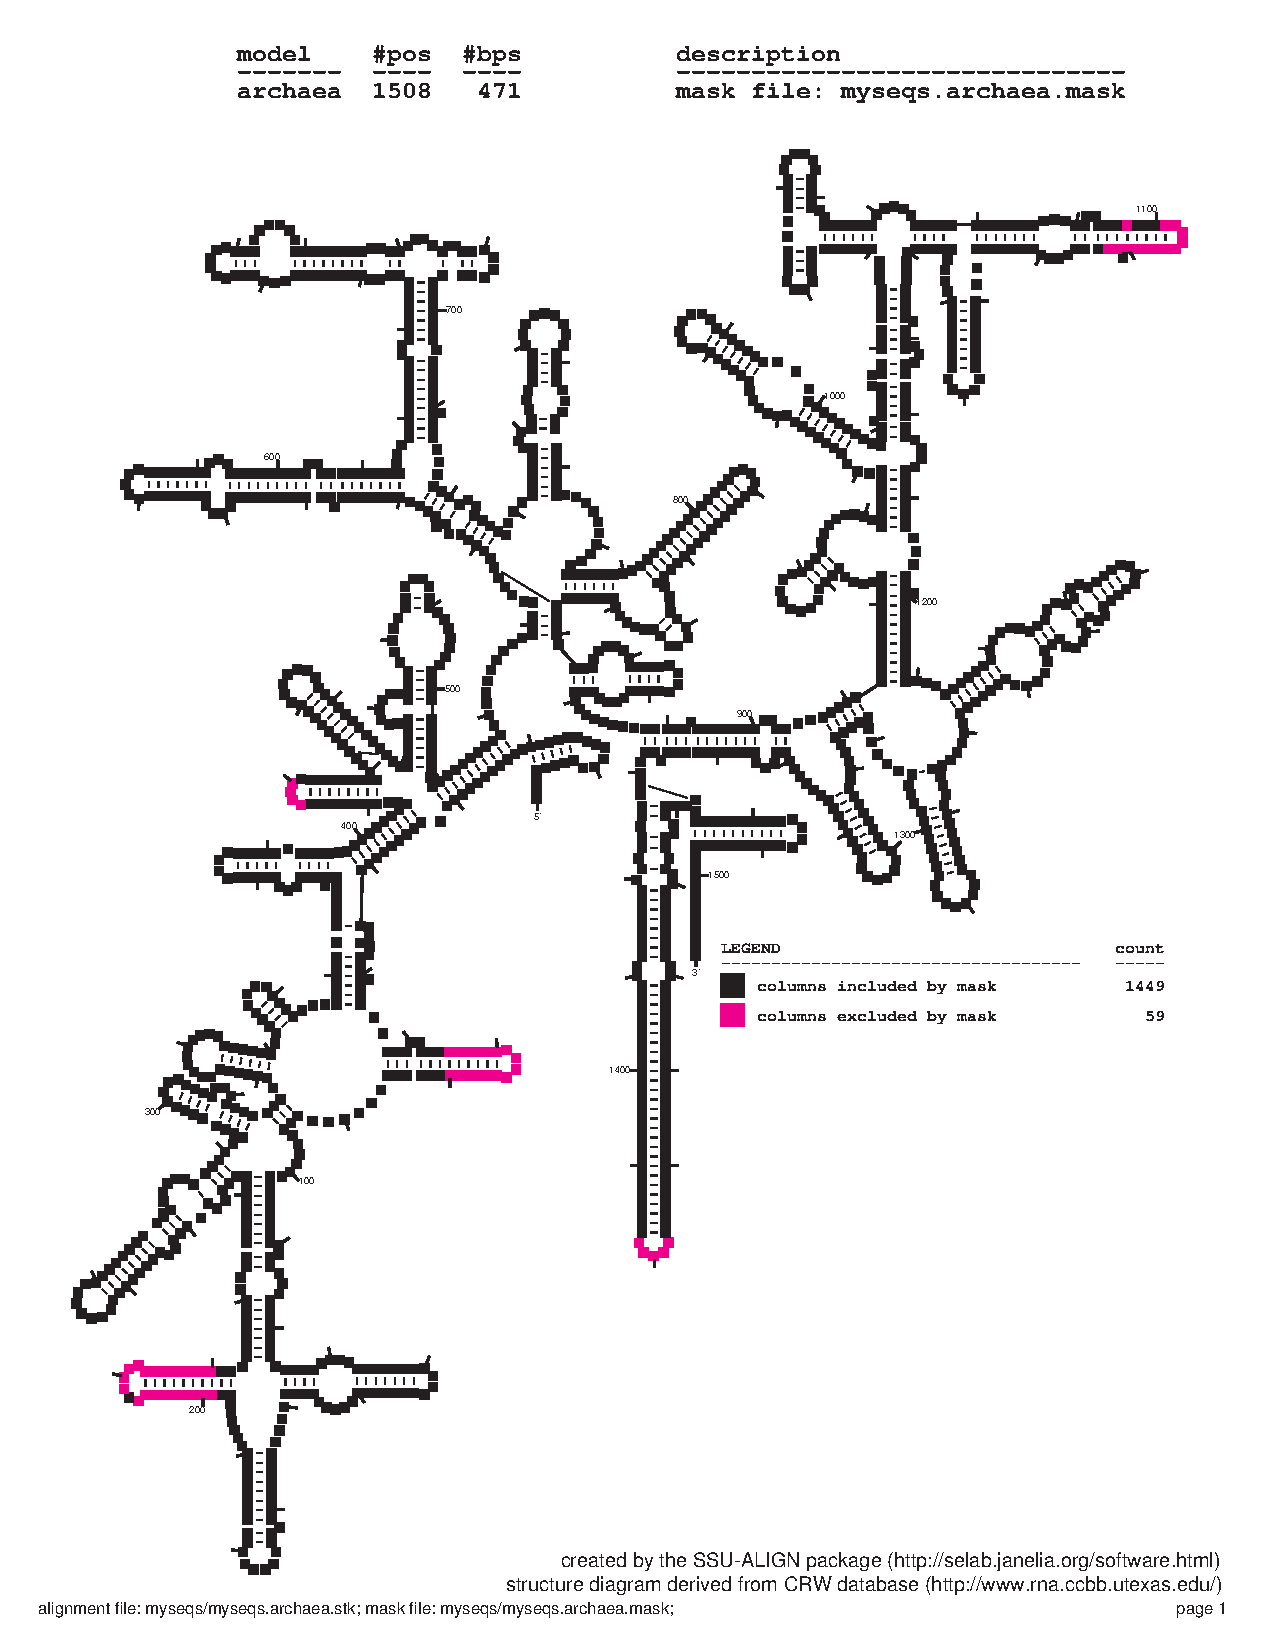
\includegraphics[width=6.5in]{Figures/myseqs-archaea-mask}
\textbf{Archaeal posterior probability-based mask for the tutorial example.}
  \end{center}
\label{fig:myseqs-archaea-mask}
\end{figure}

\subsubsection{using precalculated masks for consistent masking of
  multiple datasets}

In the \prog{ssu-mask} example above, we calculated a mask
specifically based on our \prog{myseqs} alignments. Given a different
dataset of SSU sequences, the generated masks would very likely be
different (i.e. exclude different columns). This
per-alignment-specificity can be undesirable. For example, if you'd
like to directly compare alignments from multiple runs of
\textsc{ssu-align} you probably want to make sure all of the
alignments being compared contain an identical set of consensus
positions \footnote{This would also allow the alignments to be combined
easily; see the \prog{ssu-merge} manual page.}. \textsc{ssu-align}
contains a default, precalculated mask for each of the three
models. These masks were derived from very large alignments as
described in section X (TO DO). As we'll see in the next example, you
can use these masks by supplying the \prog{-d} option to
\prog{ssu-mask}. We'll also use the \prog{--key-out} option to add the
string 'default' to the names of the output files so we do not
overwrite the files we created in the previous example. This option
enables you to save multiple sets of alignments and masks in a single
directory:

\user{ssu-mask -d --key-out default myseqs}

\begin{sreoutput}
# Masking alignments using pre-existing masks...
#
#                                                    mask    
#                                                ------------
# file name                 in/out  type  #cols  incl.  excl.
# ------------------------  ------  ----  -----  -----  -----
  myseqs.archaea.stk         input   aln   1511      -      -
  archaea-0p1.mask           input  mask   1508   1376    132
  myseqs.archaea.mask.pdf   output   pdf   1508   1376    132
  myseqs.archaea.mask.stk   output   aln   1376      -      -
#
  myseqs.bacteria.stk        input   aln   1597      -      -
  bacteria-0p1.mask          input  mask   1582   1376    206
  myseqs.bacteria.mask.pdf  output   pdf   1582   1376    206
  myseqs.bacteria.mask.stk  output   aln   1376      -      -
#
  myseqs.eukarya.stk         input   aln   2009      -      -
  eukarya-0p1.mask           input  mask   1881   1343    538
  myseqs.eukarya.mask.pdf   output   pdf   1881   1343    538
  myseqs.eukarya.mask.stk   output   aln   1343      -      -
\end{sreoutput}

The output is similar to the previous example, but note that the
\prog{.mask} suffixed files were input rather than output (these files
are placed in your \$SSUALIGNDIR during installation), and the number
of columns included and excluded has changed.

There are several other options that can be supplied to
\prog{ssu-mask}, including \prog{-s} and \prog{-k} which let you 
use your own precalculated masks. See the \prog{ssu-mask}
manual page for more information. 

\subsubsection{converting Stockholm alignments to FASTA format}
Once the ambiguously aligned regions of the alignment are removed you may
want to use the alignments as input to a phylogenetic inference
program. However, not many of those programs accept Stockholm formatted
alignments as input. You can convert the Stockholm alignments to aligned FASTA
using the \prog{ssu-mask} program by specifying the \prog{--stk2afa}
option on the command line:

\user{ssu-mask --stk2afa myseqs}

After running, three \prog{.afa} suffixed files will have been created
in the \prog{myseqs} directory.






\subsection{Visualizing alignments with \sft{esl-ssudraw}}

SSU rRNA alignments are large and difficult to view in a meaningful
way. The \prog{esl-ssudraw} program introduced for visualizing masks
earlier in this tutorial can be also used to display statistics of
a particular alignment on the consensus SSU secondary structure of the
model used to create the alignment. As before,
using \prog{esl-ssudraw} requires a template postscript file of the
consensus secondary structure. The template files for the 3 default
\textsc{ssu-align} version 0.1 seed models are included as
\prog{\$INFDIR/ssu-align-0.1/seeds/ss-diagrams/{archaea,bacteria,eukarya}-0p1.ps}. 
(Unfortunately, it is difficult to create new template files for
additional models you might build for your own analyses.) 

\prog{esl-ssudraw} can be run in two different modes. In the default
mode, \emph{alignment} mode, the structure diagrams will display
statistics on the alignment. In \emph{individual} mode, the structure
diagrams will show individual sequences in the alignment by displaying
the actual residues at each consensus position of the alignment. Note
that the diagrams are always of the consensus model defined in the
template file. In alignment mode, only statistics of consensus
positions are displayed. In individual mode, only residues that align to
consensus positions are displayed.

The following table summarizes the different statistics that can be
created in alignment mode.
An example of each of these types of
diagrams is included as the indicated figure for the default
eukaryotic seed alignment. The postscript and pdf files for each of
these included figures, as well as analogous diagrams for the
archaeal and bacterial seeds are included in 
\prog{\$INFDIR/ssu-align-0.1/seeds/ss-diagrams/}, named as indicated 
in the ``file'' column of the table. 

\begin{center}
\begin{tabular}{llll} \hline
\prog{esl-ssudraw} option(s) & statistic                     &  figure & file \\ \hline
\prog{<none>}                & information content           & \ref{fig:eukinfo} & \prog{eukarya-0p1-info} \\
& & & \\
\prog{--prog}                & average posterior probability & \ref{fig:eukprob} & \prog{eukarya-0p1-prob} \\
& & & \\
\prog{--ins}                 & frequency of insertions       & \ref{fig:eukins}   & \prog{eukarya-0p1-ins} \\
                             & after each position           & & \\
& & & \\
\prog{--dall}                & frequency of deletions        & \ref{fig:eukdall}  & \prog{eukarya-0p1-dall} \\
& & & \\
\prog{--dint}                & frequency of internal deletions & \ref{fig:eukdint}  & \prog{eukarya-0p1-dint} \\
                             & (excluding terminal deletions)  & & \\
& & & \\
\prog{--struct}              & additional information from     & \ref{fig:eukstruct} & \prog{eukarya-0p1-struct} \\
                             & conserved structure \\
\end{tabular}
\end{center}

As an example of how these files were created, the command

\user{esl-ssudraw --dall eukarya-0p1.stk eukarya-0p1.ps eukarya-0p1-dall.ps}

was used to create Figure~\ref{fig:eukdall} (after copying the seed alignment
in \prog{\$INFDIR/ssu-align-0.1/seeds/eukarya-0p1.stk} and the template file 
\prog{\$INFDIR/ssu-align-0.1/seeds/ss-diagrams/eukarya-0p1.ps} to the current 
working directory.)

\newpage

\begin{figure}
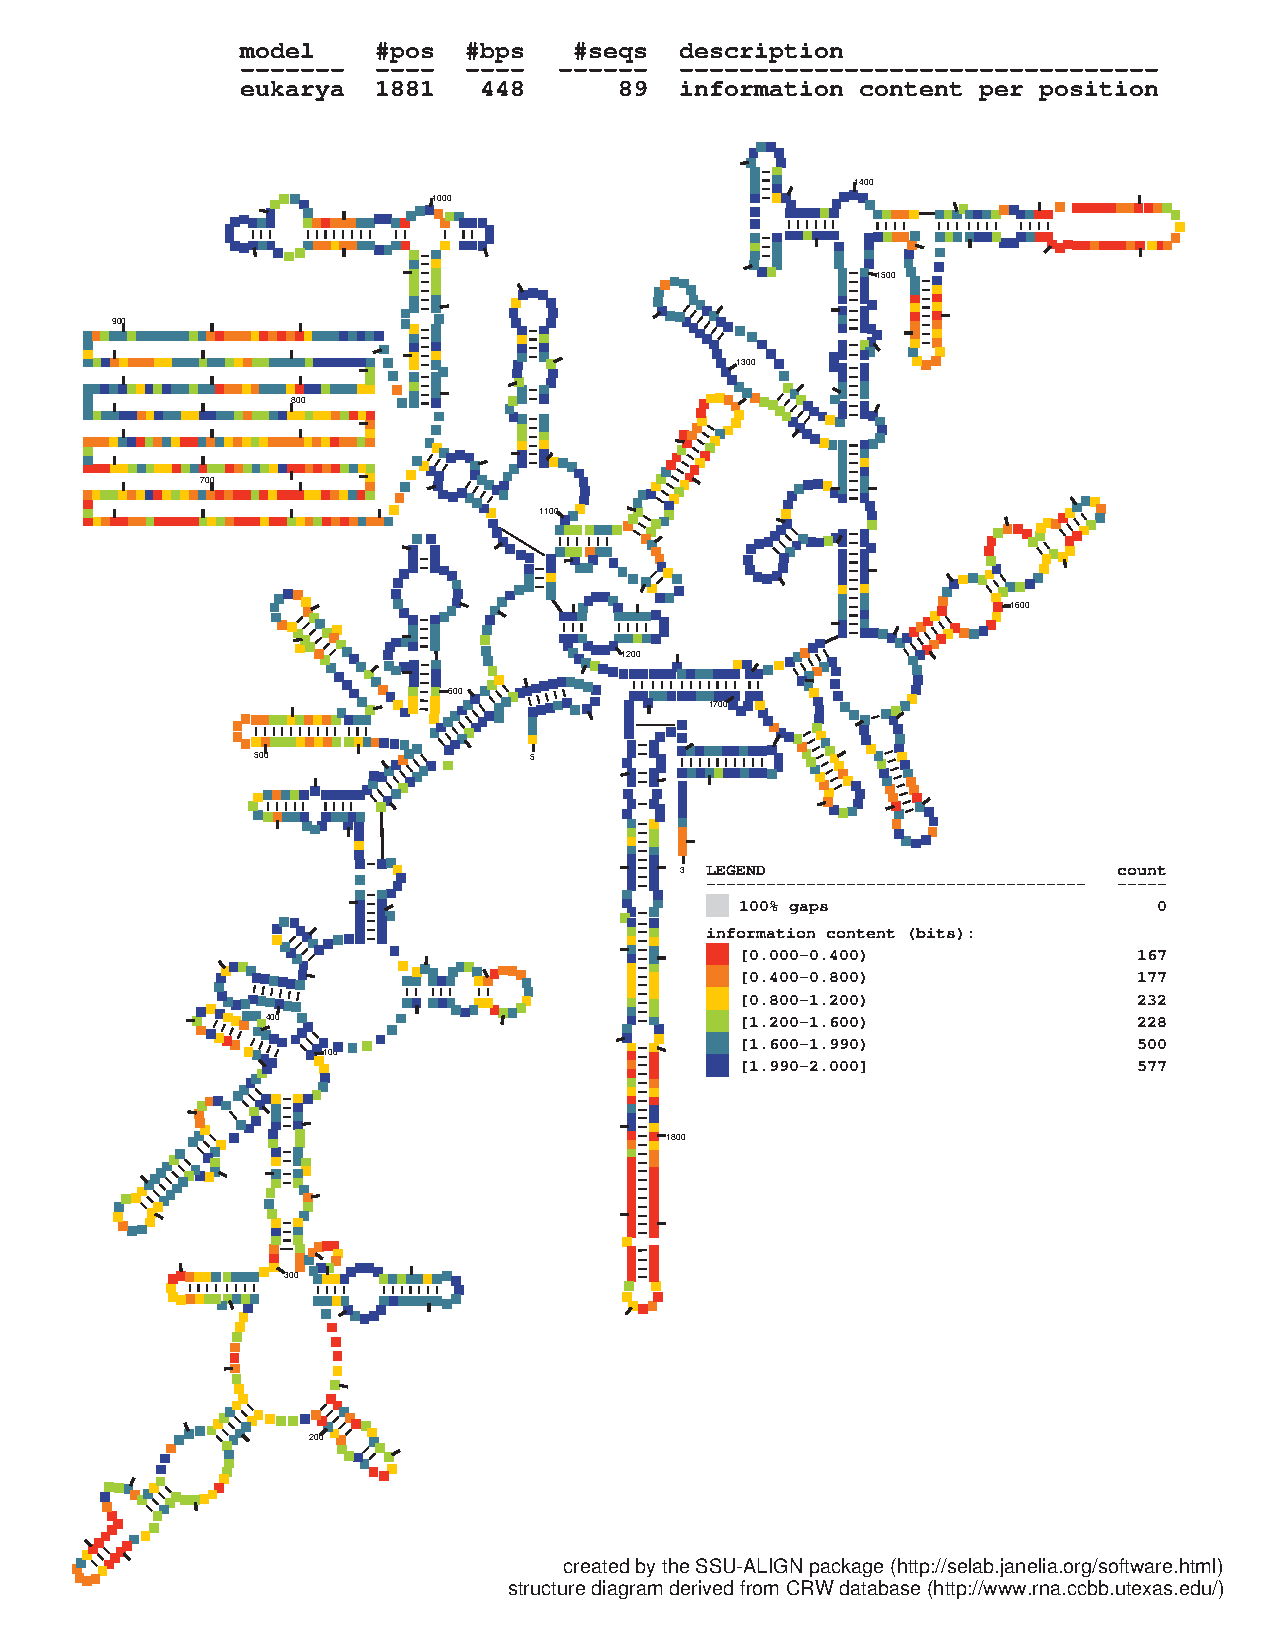
\includegraphics[height=8.5in]{Figures/eukarya-0p1-info}
\label{fig:eukinfo}
\end{figure}

\newpage

\begin{figure}
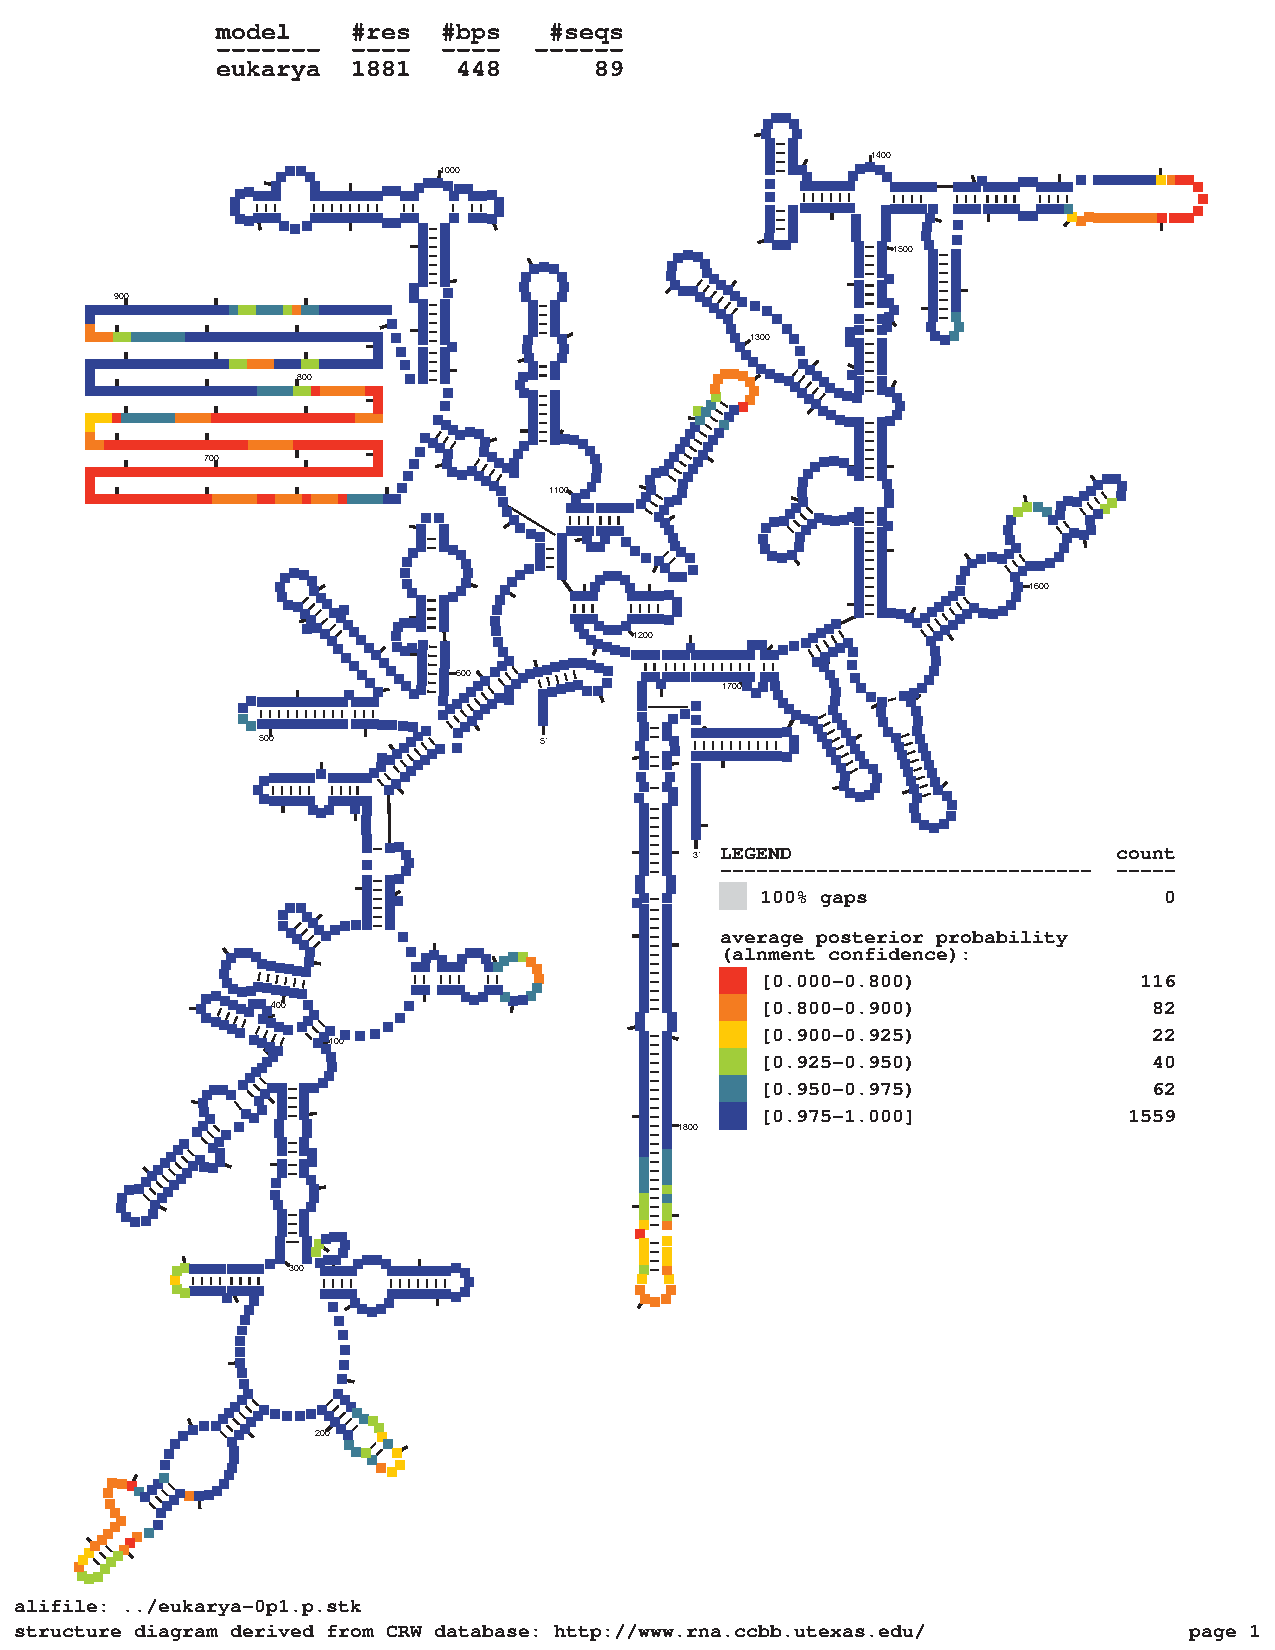
\includegraphics[height=8.5in]{Figures/eukarya-0p1-prob}
\label{fig:eukinfo}
\end{figure}

\newpage

\begin{figure}

\includegraphics[height=8.5in]{Figures/eukarya-0p1-ins}
\label{fig:eukinfo}
\end{figure}

\newpage

\begin{figure}
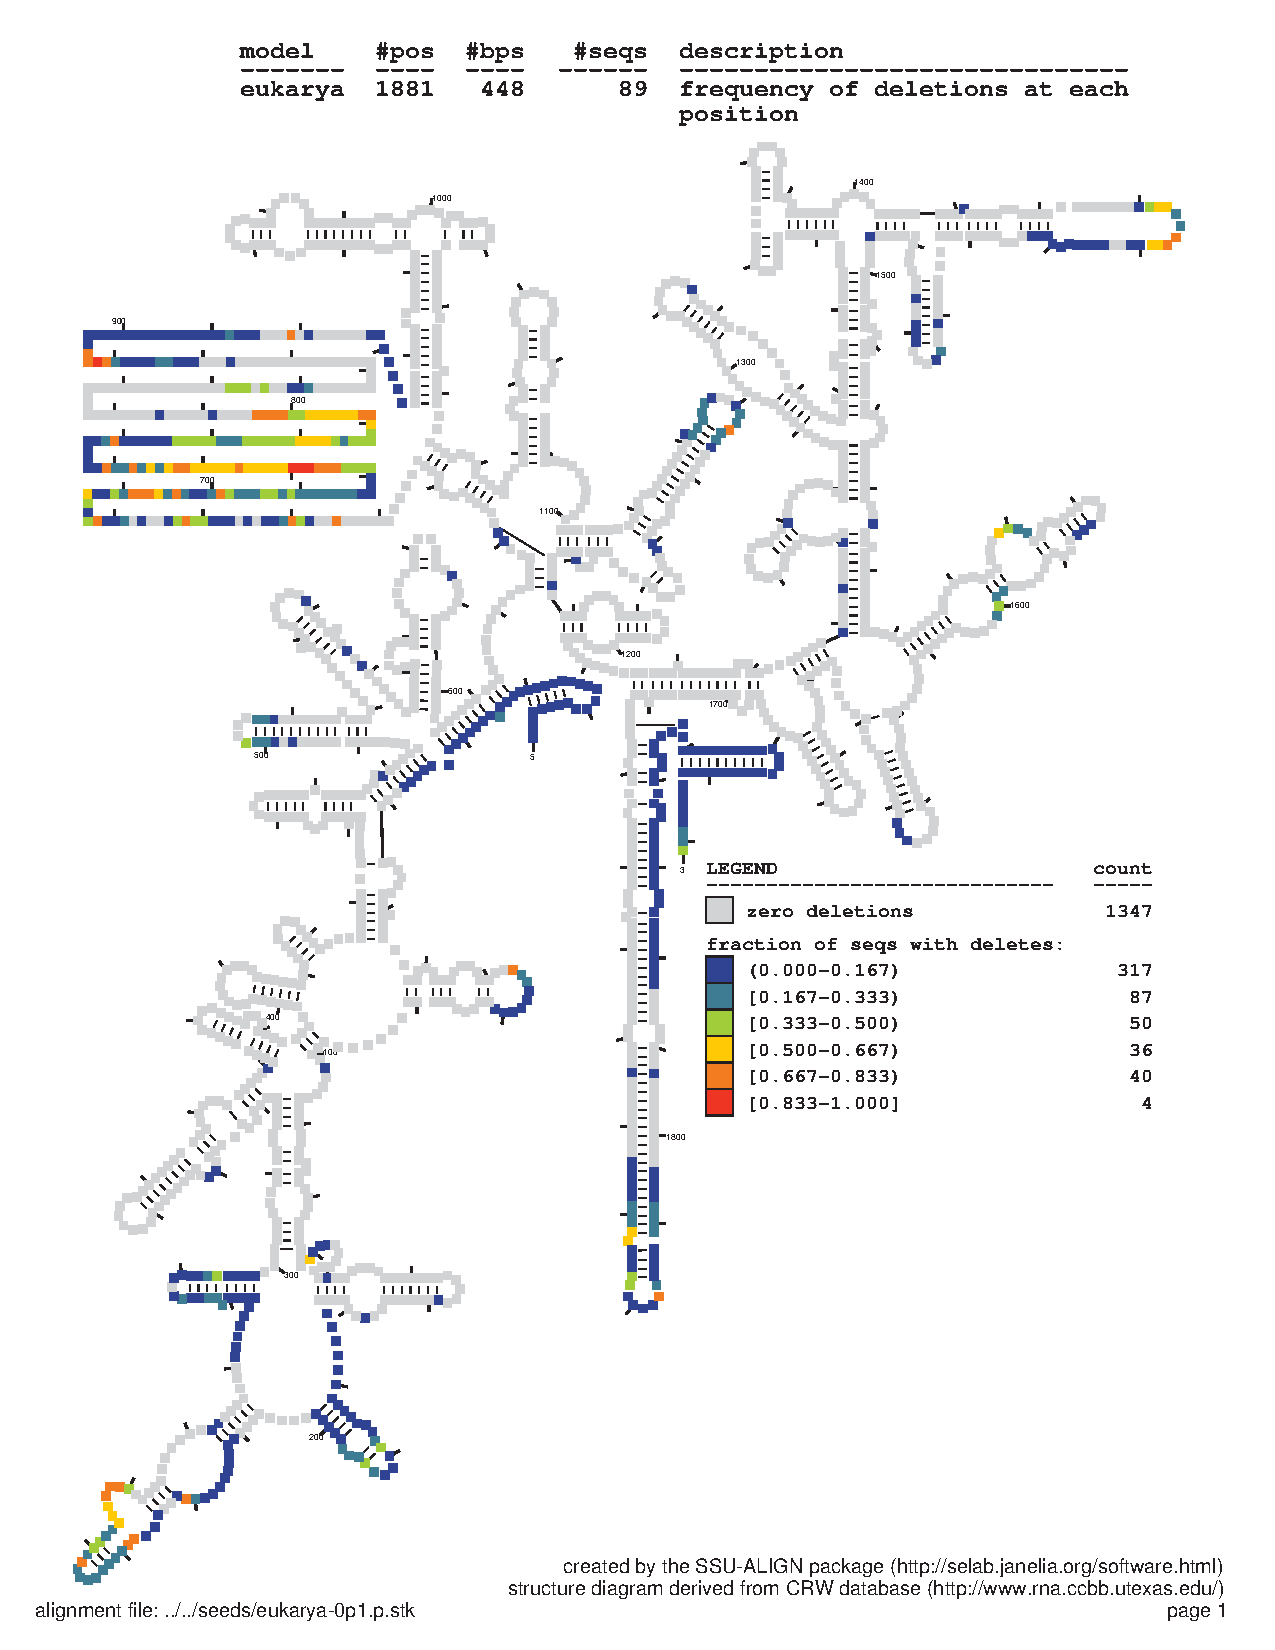
\includegraphics[height=8.5in]{Figures/eukarya-0p1-dall}
\label{fig:eukinfo}
\end{figure}

\newpage

\begin{figure}
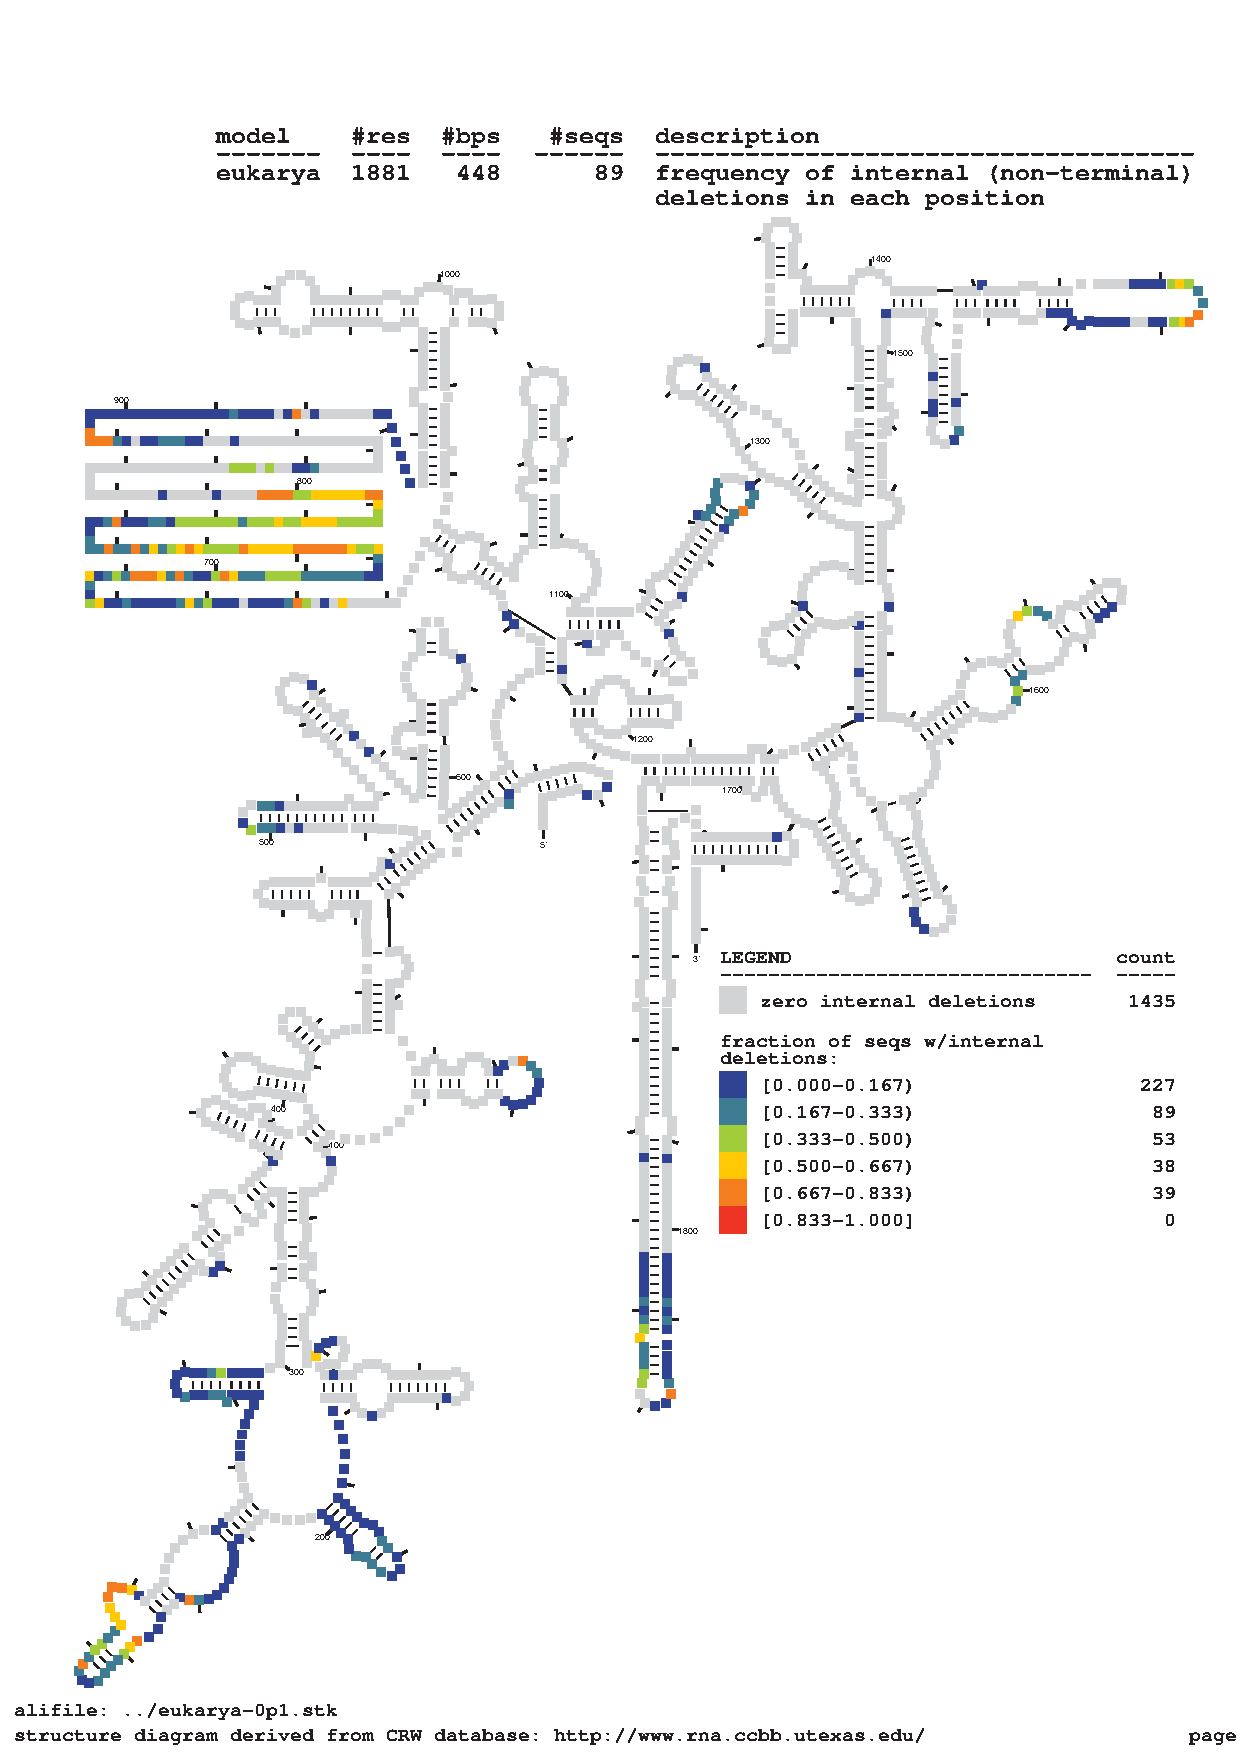
\includegraphics[height=8.5in]{Figures/eukarya-0p1-dint}
\label{fig:eukinfo}
\end{figure}

\newpage

\begin{figure}
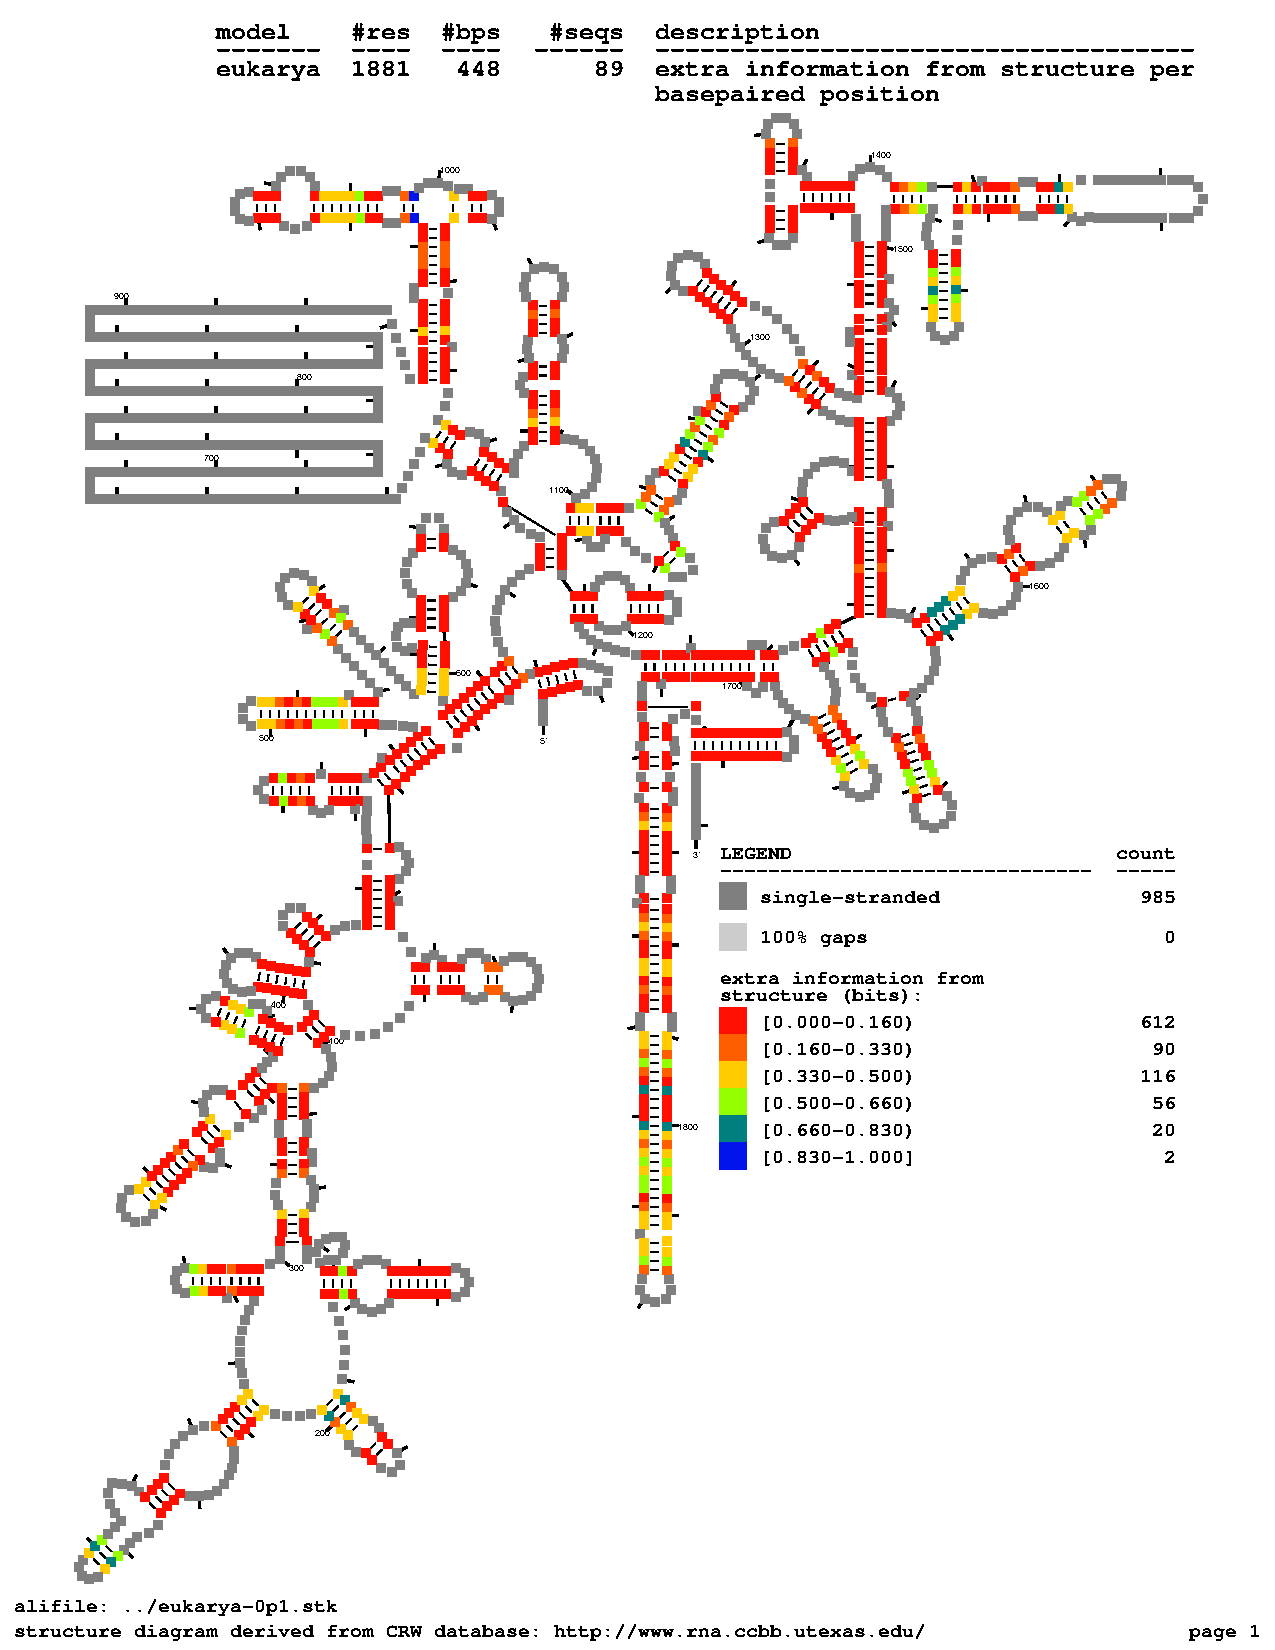
\includegraphics[height=8.5in]{Figures/eukarya-0p1-struct}
\label{fig:eukinfo}
\end{figure}








\subsection{Using ssu-build to create a truncated model of a specific region of SSU rRNA}

Many SSU rRNA sequencing studies target a specific region of the SSU
rRNA molecule using PCR primers at the boundaries of that region. For
such studies it is recommended to build a new CM that only models the
region of the molecule targeted by the study. There are two reasons
for this. The first is speed: the running time of \textsc{ssu-align}
decreases as the model size it's using decreases. The second reason is
that aligning a SSU subsequence to a model of only the region that
subsequence is derived from, relative to a model of the entire SSU
molecule, should slightly increase alignment accuracy. This is because
the uncertainty regarding what region of the full molecule the subsequence
should align to is eliminated. In this section I'll demonstrate how to
create a CM of a specific region of SSU and use it to create
alignments. 

In this example, we'll build three new CMs targetted to the so-called
V4 hypervariable region, one each for archaea, bacteria and
eukarya. We'll use the \textsc{ssu-align} default seed alignments that
were used to create the default full-length CMs. 

The first step is to identify the region of each of the three default
models we want our new models to represent. The secondary structure
diagrams in the \prog{seeds/ss-diagrams/} subdirectory of the
{ssu-align-0.1/} directory where you unpacked the package.
In particular, the files suffixed with \prog{.rf.pdf} and
\prog{.info.pdf} are probably most useful. These figures are included
in this guide in section~\ref{sec:models} as
figures~\ref{fig:archaea-rf} and \ref{fig:archaea-info} (archaea),
\ref{fig:bacteria-rf} and \ref{fig:eukarya-info} (bacteria),
\ref{fig:eukarya-rf} and \ref{fig:eukarya-info} (eukarya).
In these figures, every 100th position is numbered, and every 10th
position is indicated by a tick mark.

Based on the bacterial primer sites used by a recent environmental
study that targetted the V4 region \cite{Claesson09}, I determined 
the V4 region in the default bacterial model spans positions 584
through 824, via manual inspection of the bacterial secondary structure
diagrams. By comparison to the archaeal and eukaryal diagrams, 
the corresponding region in archaea is from positions 525 to
765, and in eukarya is 620 to 1082. 

Given these coordinates, we can use \prog{ssu-build} to create V4
specific models. 
First, create and move into a new directory where we'll build the new
models. For example, from the \prog{tutorial/} directory, do:

\user{mkdir myv4; cd myv4}

The models must be built one at a time. First, we'll
create the archaeal v4 model:

\user{ssu-build -d --trunc 525-765 -n arc-v4 -o v4.cm archaea}

The \prog{-d} option tells \prog{ssu-build} to use a default model,
\prog{--trunc 525-765} specifies the positions of the model, \prog{-n arc-v4}
specifies the name of the model should be \prog{arc-v4} and \prog{-o
  v4.cm} specifies the name of the CM file be \prog{v4.cm} (we'll add
two more models to this file next). Finally, \prog{archaea} tells the
program to use the default archaeal model. As with the other programs,
\prog{ssu-build} reports on what it's doing:

\begin{sreoutput}
# Truncating alignment and default mask; saving only columns between predefined consensus
# columns 525 and 765...
#
# output aln file           
# --------------------------
  archaea-0p1-sb.525-765.stk
#
# truncated mask file name   
# ---------------------------
  archaea-0p1-sb.525-765.mask
#
# Building CM(s)...
#
#                           num  alignment  consensus   num
# CM file name  CM name    seqs     length     length   bps
# ------------  -------  ------  ---------  ---------  ----
  v4.cm         arc-v4       23        242        241    69
#
# structure diagram file    
# --------------------------
  archaea-0p1-sb.525-765.pdf
#
\end{sreoutput}

Several files have been created:

\begin{sreitems}{}

\item[\prog{archaea-0p1-sb.525-765.stk}] the region of the default
  archaeal seed alignment spanning consensus columns 525 to
  765. This alignment was used to build the new archaeal V4 model.
  
\item[\prog{archaea-0p1-sb.525-765.mask}] the region of the default
  archaeal mask (see section~\ref{sec:masks}) spanning consensus
  columns 525 to 765. This mask file could potentially be useful to mask
  alignments created using the new archaeal v4 model with the
  \prog{ssu-mask} option and the \prog{-s} option.
  
\item[\prog{v4.cm}] the CM file with the new archaeal V4 model named
  \prog{arc-v4}. As indicated by the output, the model was built
  from an alignment of width 242 positions that included 69
  basepairs of 23 archaeal sequences (the region of the default
  archaeal alignment spanning from consensus positions 525 to 765).
  
\item[\prog{archaea-0p1-sb.525-765.ps}] a structure diagram 
  of the archaeal consensus model highlighting the region from
  positions 525 to 765 represented by the new model in \prog{v4.cm}.
  This diagram is included as figure~\ref{fig:v4}.
\end{sreitems}

Next we'll build bacterial v4 and eukaryal v4 models and append them
to the \prog{v4.cm} file:

\user{ssu-build -d --trunc 584-824 -n bac-v4 --append v4.cm bacteria}

\user{ssu-build -d --trunc 620-1082 -n euk-v4 --append v4.cm eukarya}

The \prog{--append} option tells \prog{ssu-build} to append the new model
onto the existing file \prog{v4.cm}.
After executing these two commands, the \prog{v4.cm} file will contain
three v4 models. This CM file can be used to create domain-specific
SSU v4 alignments from a set of SSU sequences using
\prog{ssu-align}. An example dataset this would be particularly useful
for would be a set of SSU sequences generated from an environmental
sequencing survey that used three sets of PCR primers: one each for
the archael, bacterial and eukaryal v4 regions. Alternatively, it
could be used to create v4-only alignments from a set of full length
SSU sequences. We'll demonstrate the latter application here using our
sample dataset from earlier in the tutorial in the file:
\prog{tutorial/seed-15.fa}, which contains 5 full or nearly-full
length archaeal, bacterial and eukaryotic SSU sequences:

\prog{ssu-align -m v4.cm ../seed-15.fa myv4seqs}\footnote{This assumes your
  current working directory is in a subdirectory of \prog{tutorial/},
  if it's not specify the correct path to the \prog{seed-15.fa} file
  in the \prog{tutorial} subdirectory of \prog{ssu-align-0.1}.}

The \prog{-m} option specifies that the model \prog{v4.cm} be used. 
Using this model, processing \prog{seed-15.fa} takes only about 4
seconds, as opposed to the 20 seconds it took with the default,
full-length models earlier in the tutorial. Take a look at
\prog{myv4seqs/myv4seqs.bacteria.stk}, it contains only the v4 regions
of the 5 bacterial sequences from \prog{seed-15.fa}. 

As with the earlier example, these alignments can be masked with the
\prog{ssu-mask} program, though I won't step through that
here. However, the \prog{ssu-draw} program cannot be used to draw
diagrams of alignments created using any models other than the default
three, so it is not possible to create drawings of these alignments.


\begin{sidewaysfigure}
  \begin{center}
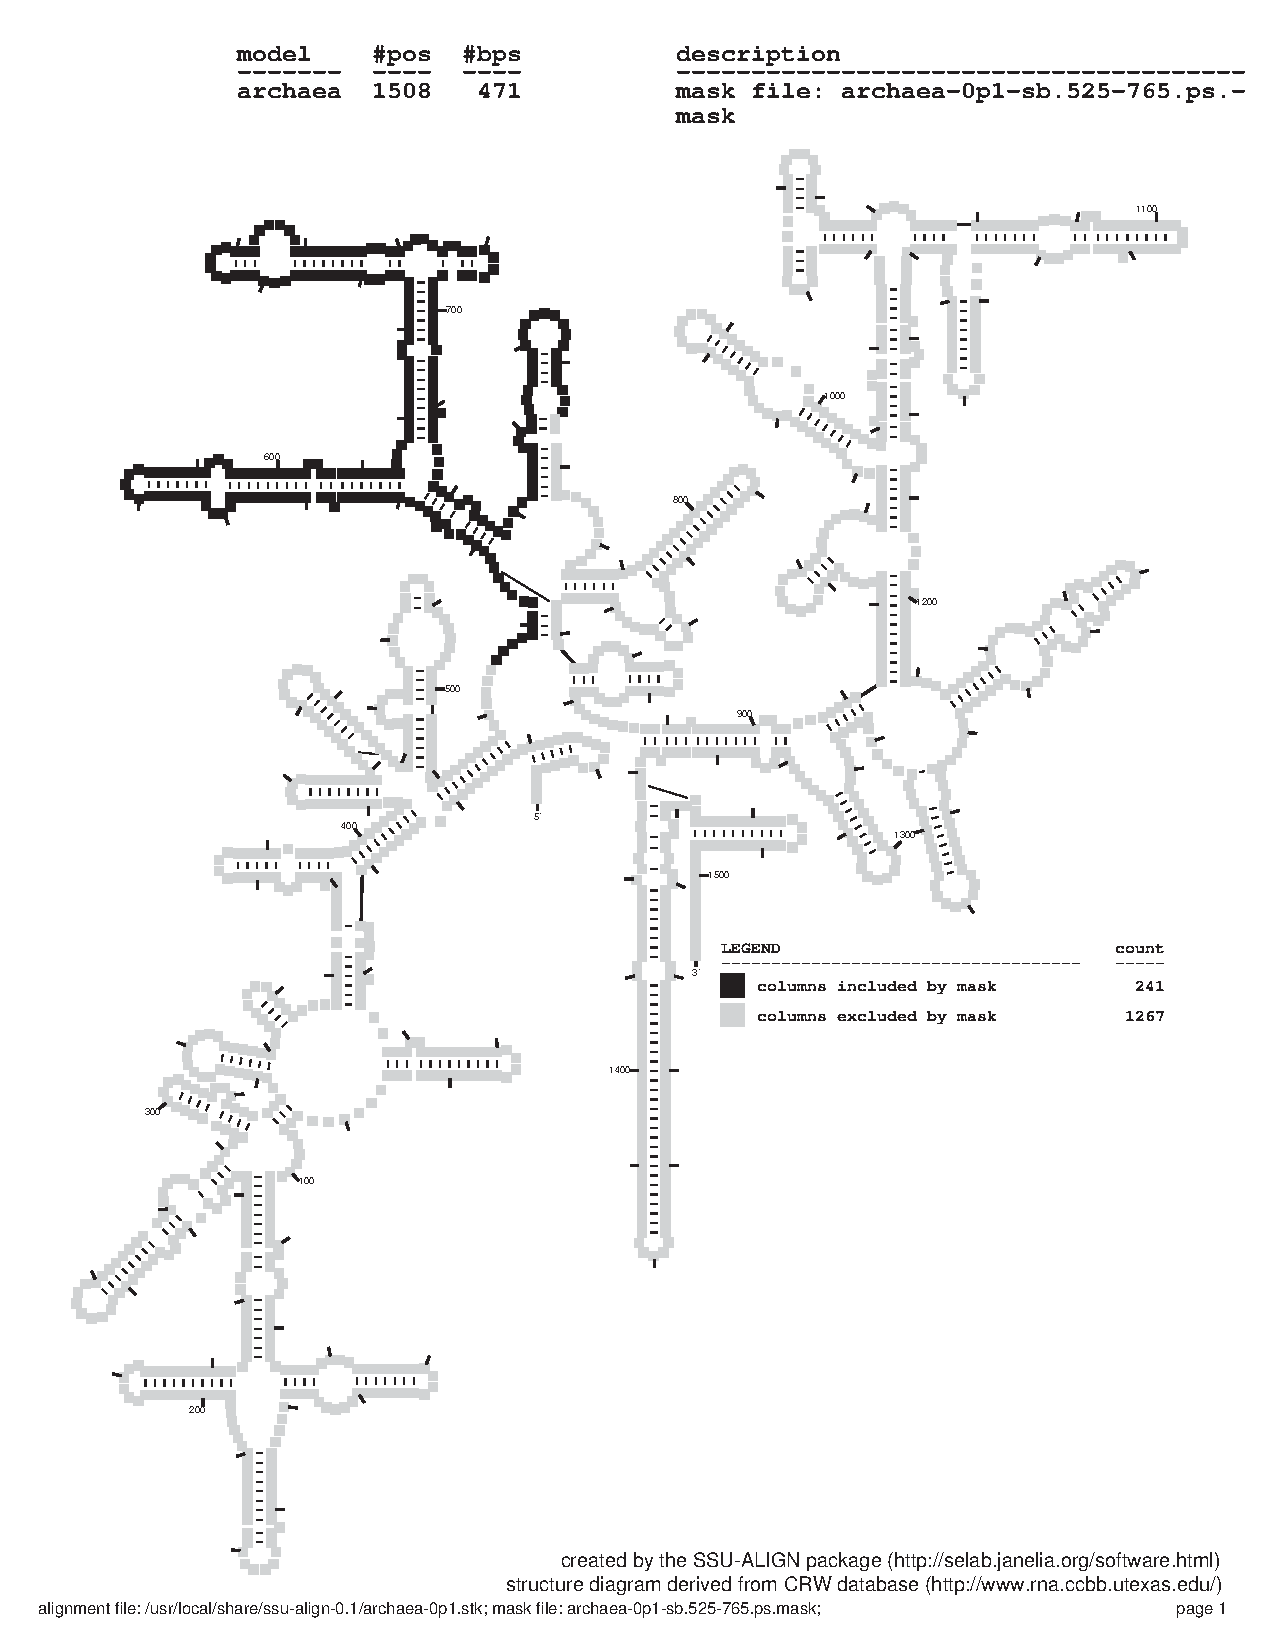
\includegraphics[width=2.8in]{Figures/arc-v4}
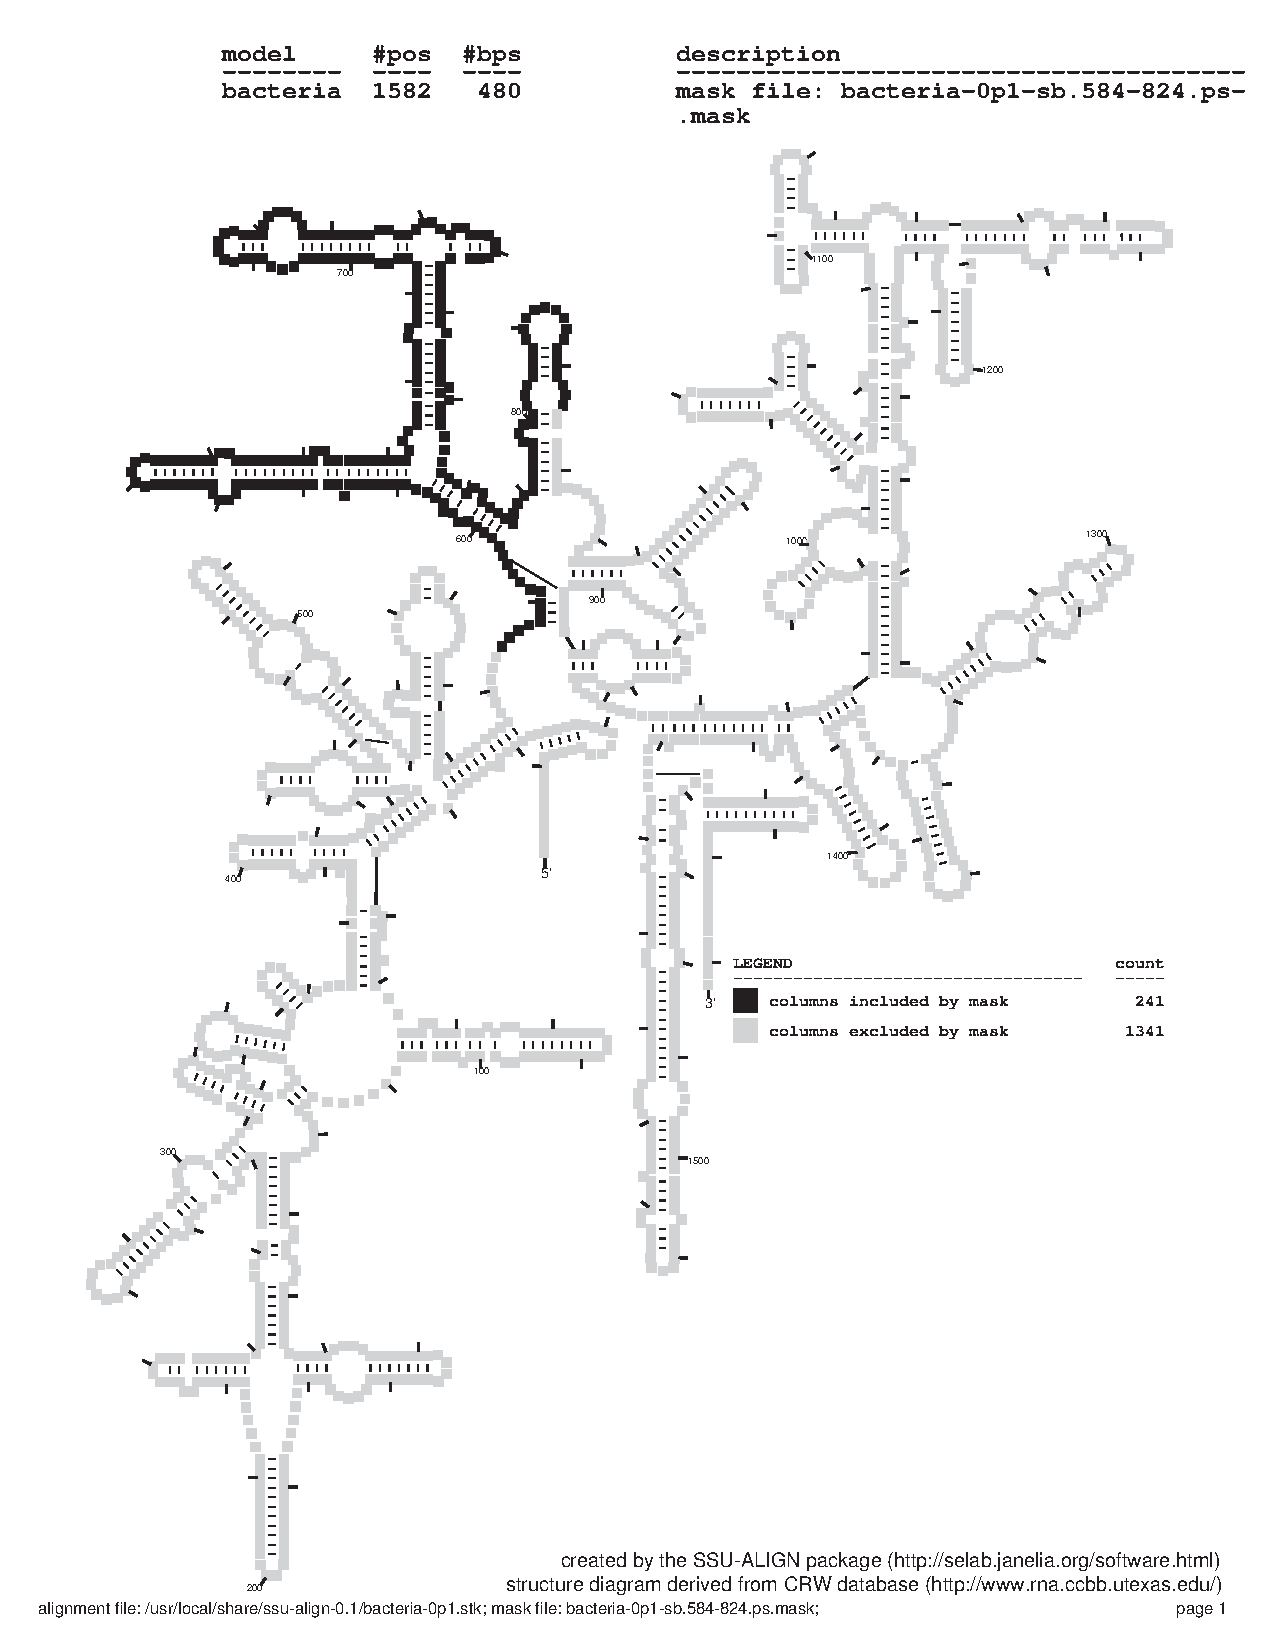
\includegraphics[width=2.8in]{Figures/bac-v4}
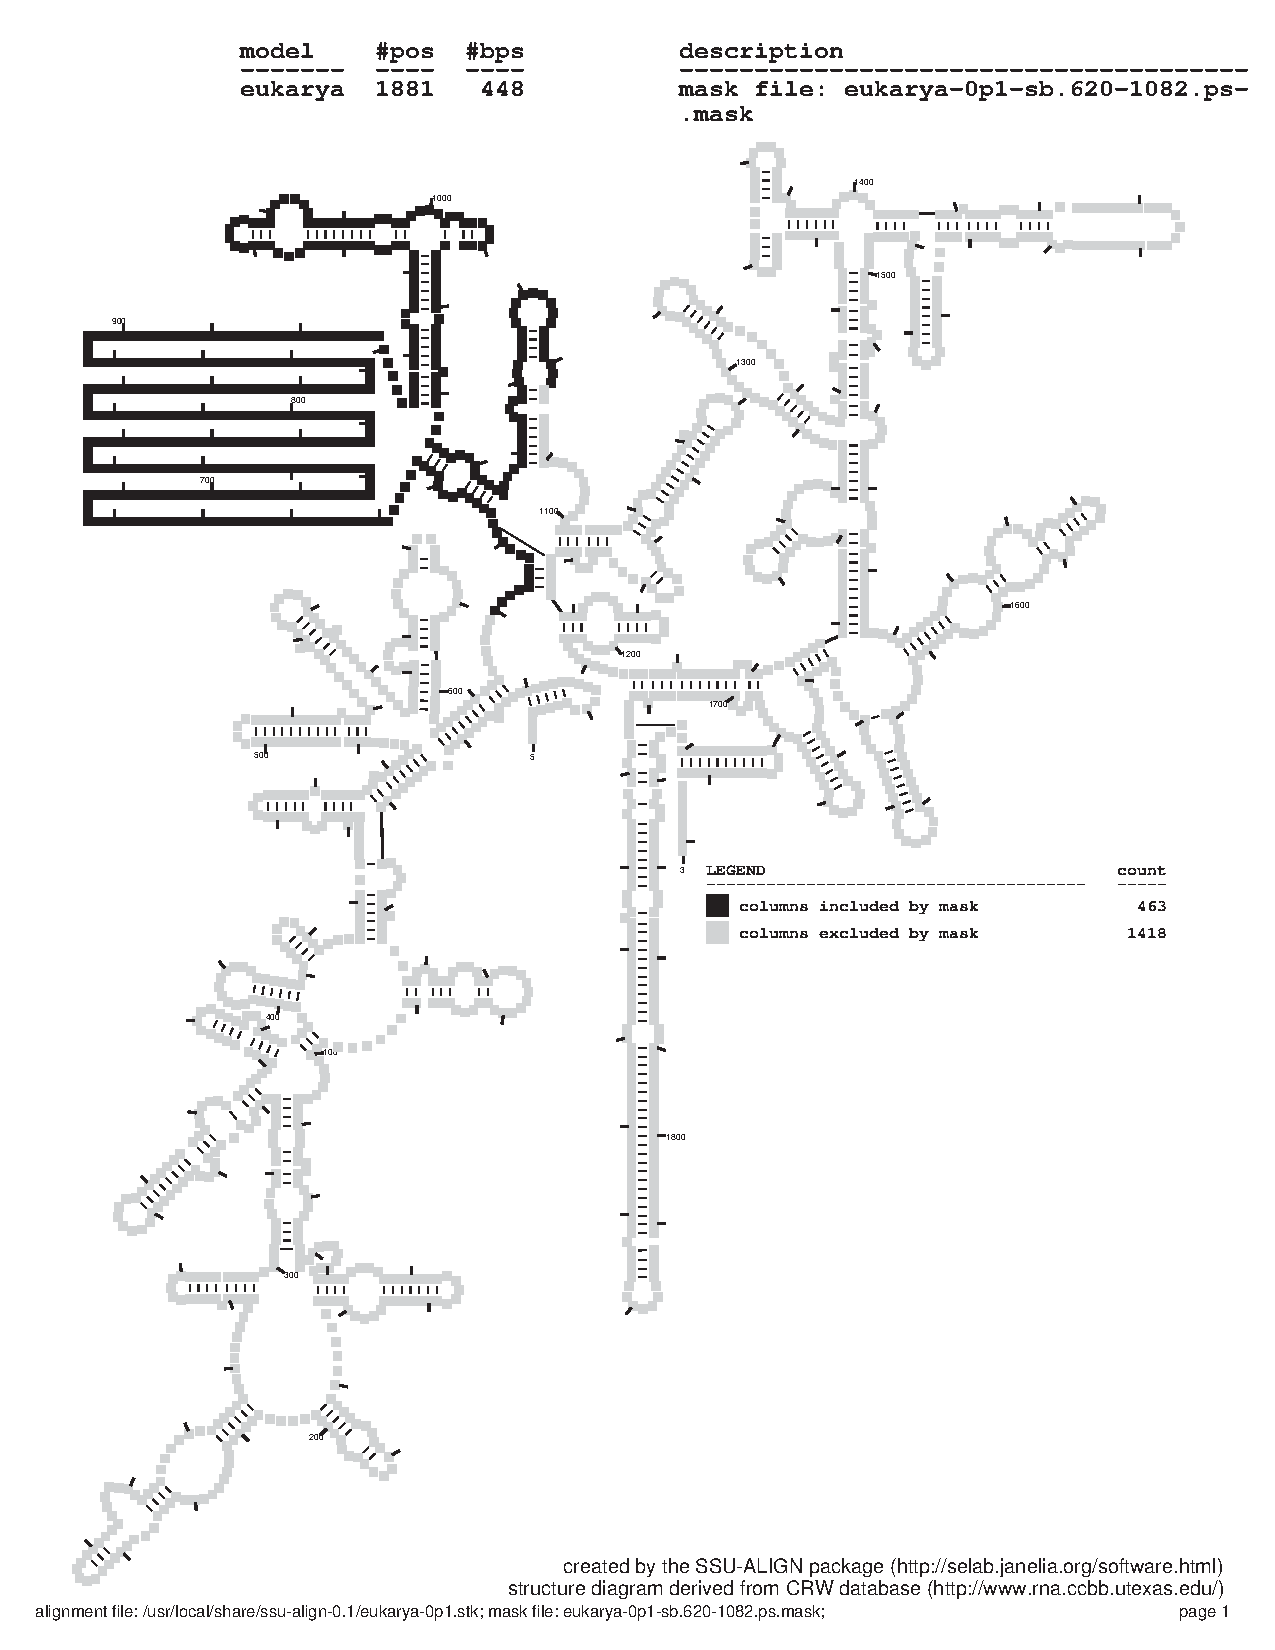
\includegraphics[width=2.8in]{Figures/euk-v4}

\textbf{V4 regions in archaea (left), bacterial (middle) and eukarya
  (right).} These diagrams are generated by \prog{ssu-build} in the
  tutorial.
  \end{center}
\label{fig:v4}
\end{sidewaysfigure}


\subsection{Faster alignment of large datasets through parallelization
  with ssu-prep}
\label{sec:tutorial-prep}
\prog{ssu-align} runs on a single processor and does not support MPI
or multi-threading. However, if you have access to a compute
cluster or multi-core computers, simplistic parallelization is possible
with the \prog{ssu-prep} program.

\prog{ssu-prep} will split up a large input sequence file into
\emph{n} smaller files and create a shell script that will execute
\emph{n} \prog{ssu-align} jobs in parallel, each processing one of the
small sequence files. The results of all jobs will automatically be
merged together by the final job, ultimately yielding the same results
as if a single 
\prog{ssu-align}
job was run for the original large input sequence file. 
Parallelizing \prog{ssu-align} in this way can drastically reduce the
actual time required for aligning large datasets. A job that would
have required 100 hours on 1 processor can be done in a little more
than 1 hour on 100 processors. See table~\ref{tbl:ttimes} in
section~\ref{sec:stats} for example timing statistics. 

In this section we'll walk through an example of how to do this for a
small dataset.  The sequence file \prog{tutorial/seed-30.fa} includes
30 randomly chosen sequences from the complete set of seed sequences
from the three default models of \textsc{ssu-align}.

\prog{ssu-prep} has three different usage modes as explained by the
program if it is run without any command-line arguments:

\user{ssu-prep}

\begin{sreoutput}
Incorrect number of command line arguments.
Usage: ssu-prep    [-options] <seqfile> <output dir> <num jobs> <prefix/suffix file>
Usage: ssu-prep -x [-options] <seqfile> <output dir> <num jobs>
Usage: ssu-prep -y [-options] <seqfile> <output dir> <num jobs>

ssu-prep splits up <seqfile> into <num jobs> smaller files and creates a shell
script that will execute <num jobs> ssu-align jobs in parallel, each processing
one of the small sequence files. The results of all jobs will automatically be
merged together by the final job, giving the same results as if a single
ssu-align job was run for the complete <seqfile>.

The 3 different usages control how the prefix and suffix are defined for the jobs
in the output shell script, allowing, for example, the user to wrap the ssu-align
commands in a cluster submission command (such as Sun Grid Engine's "qsub"):

Default: (neither -x nor -y enabled) prefix and suffix for ssu-align jobs in
         output shell script are defined in <prefix/suffix file>. First line is
         the prefix, second line is the suffix.
With -x: do not specify <prefix/suffix file>; output shell script will run all
         <num jobs> jobs in parallel on one machine with <num jobs> cores/cpus.
With -y: do not specify <prefix/suffix file>; user will manually add the desired
         prefix/suffix to ssu-align commands after ssu-prep finishes.

To see more help on available options, do ssu-prep -h
\end{sreoutput}

By default, if neither \prog{-x} nor \prog{-y} options are used, the program
reads a \prog{<prefix/suffix file>}, a simple two line file that
a prefix string and a suffix string to prepend and append respectively
to the \prog{ssu-align} commands it generates. 

The strings in the \prog{<prefix/suffix file>} will likely be specific
to your parallel computing environment. At Janelia, we use Sun Grid
Engine's \prog{qsub} program for submitting jobs to a large compute
cluster. The relevant prefix/suffix file for our specific
computing environment is included in \\
\prog{tutorial/janelia-cluster-presuf.txt}. Take a look at this file:

\begin{sreoutput}
qsub -N ssu-align -o /dev/null -b y -j y -cwd -V "
"
\end{sreoutput}

The first line is the prefix string, containing the name and
appropriate command line arguments of the \prog{qsub} program which
submits jobs to the Grid Engine queuing system at Janelia. The second
line is the suffix, and contains only a double quote, which
complements the double quote at the end of the prefix line as we'll
see below.

Now, let's run \prog{ssu-prep} as if we were going to create parallel
\prog{ssu-align} jobs for the Janelia cluster.  Move into the
\prog{tutorial/} directory and execute the command:

\user{ssu-prep seed-30.fa my30 5 janelia-cluster-presuf.txt}

About forty lines of text are output to the screen. We'll step through
and discuss this output: 

\begin{sreoutput}
# Validating input sequence file ... done.
#
# Preparing 5 ssu-align jobs ...
# Partitioning seqs with goal of equalizing total number of nucleotides per job ...
#
# output file name   description                                       
# -----------------  --------------------------------------------------
  my30/seed-30.fa.1  partition 1 FASTA sequence file (6 seqs; 10463 nt)
  my30/seed-30.fa.2  partition 2 FASTA sequence file (6 seqs; 10240 nt)
  my30/seed-30.fa.3  partition 3 FASTA sequence file (6 seqs;  9922 nt)
  my30/seed-30.fa.4  partition 4 FASTA sequence file (6 seqs; 10358 nt)
  my30/seed-30.fa.5  partition 5 FASTA sequence file (6 seqs;  9397 nt)
  my30.ssu-align.sh  shell script that will execute 5 ssu-align jobs
#
\end{sreoutput}

First, \prog{ssu-prep} reports that it has validated the formatting of
the sequence file, partitioned it into 5 new files and placed each file
into the newly created \prog{my30/} subdirectory. Each of these files has
6 of the original 30 sequences in it. Additionally,
\prog{my30.ssu-align.sh}, a shell script that will execute 5 jobs, one
per sequence file, was created in the current working directory. After
this, you'll see:

\begin{sreoutput}
################################################################################
# To execute all 5 ssu-align jobs, run the shell script with:
#	sh my30.ssu-align.sh
################################################################################
\end{sreoutput}

These are instructions for how to execute the shell script. Take a
look at the shell script \\ \prog{my30.ssu-align.sh}:

\begin{sreoutput}
#!/bin/bash
# Bash shell script created by ssu-prep for running 5 ssu-align jobs.
# Each job will process a separate partition of the sequence file:
# 'seed-30.fa'.
#
# The final job is special, after computing its alignments it will wait for all
# other jobs to finish and then merge the output of all jobs together.
# The merged output files will be in the directory: '/my30/'
#
# The for loop below will execute/submit the first 4 of 5 jobs.
# The final ssu-align job is executed separately because it does the merging.
#
for i in {1..4}
do
	echo "# Executing: qsub -N ssu-align -o /dev/null -b y -j y -cwd -V " ssu-align my30/seed-30.fa.$i my30/my30.$i ""
	qsub -N ssu-align -o /dev/null -b y -j y -cwd -V " ssu-align my30/seed-30.fa.$i my30/my30.$i "
done
echo "# Executing: qsub -N ssu-align -o /dev/null -b y -j y -cwd -V " ssu-align --merge 5 my30/seed-30.fa.5 my30/my30.5 ""
qsub -N ssu-align -o /dev/null -b y -j y -cwd -V " ssu-align --merge 5 my30/seed-30.fa.5 my30/my30.5 "
\end{sreoutput}

This is a bash shell script file\footnote{The \prog{--no-bash} option
  can be used to make a non-bash-specific script, see the
  \prog{ssu-prep} manual page for more information.}.
The \prog{\#}-prefixed lines are
explanatory comments. The remainder of the file consists of a for loop
that will submit the first four \prog{ssu-align} jobs to the cluster
using \prog{qsub}. The lines beginning with \prog{qsub} are the actual
job submission commands. The lines beginning with \prog{echo} cause updates to
be printed to STDOUT before each job is submitted. 
Note that the \prog{qsub} command line is composed
of the prefix string from the \prog{janelia-cluster-presuf.txt} file,
followed by a \prog{ssu-align} command, followed by the suffix
string. The end result is that the \prog{ssu-align} command is
contained within the quotes from the prefix/suffix strings.

The comments explain that the final job is special. It will merge the
results of all jobs once they are finished. Consequently, it requires
special command-line options and so is executed outside the for loop,
as the final line of the script.

%%%%%%%%%%%%%%%%%%%%%%%%%%%%%%%%%%%%%%%%%%%%%%%%%%%%%%%%%%%%%%%%%%%%%
\begin{comment}
The final important part of the \prog{ssu-prep} output explains what
to do if any of the jobs fail: 

\begin{sreoutput}
# If one or more jobs fail: rerun the failed jobs, wait for them to finish,
# and then perform manual merge from this directory by executing:
#	ssu-merge my30
\end{sreoutput}

This should happen only rarely, but if any jobs fail, this aspect of
the program allows 
\end{comment}
%%%%%%%%%%%%%%%%%%%%%%%%%%%%%%%%%%%%%%%%%%%%%%%%%%%%%%%%%%%%%%%%%%%%%

Because your specific compute system is likely different from
Janelia's, the \prog{my30.ssu-align.sh} script will probably not
work. To make \prog{ssu-prep} generate shell scripts you can run on
your system, create a file like \prog{janelia-cluster-presuf.txt} but
with prefix and suffix strings specific to your
system. 

This simple prefix/suffix string method may not work for your
compute system. For example, if your cluster requires using \prog{ssh}
to remote login to different nodes, a single fixed prefix line will
probably not be sufficient. If this is the case, run \prog{ssu-prep}
with the \prog{-y} option. In this mode no prefix/suffix file
will be read, and the output shell script will contain only the raw
\prog{ssu-align} commands. For example, do:

\user{ssu-prep -f -y seed-30.fa my30 5}

(We had to also specify \prog{-f} so the program would overwrite our
existing \prog{my30} directory.) Much of the output is the same as the
prior example, but the \prog{WARNING} section is new:

\begin{sreoutput}
################################################################################
# WARNING: -y was set on the command line.
# This means that 'my30.ssu-align.sh' will simply run the 5 ssu-align jobs in
# succession, one after another, not in parallel. If you want to run the jobs in
# parallel you'll either have to manually edit that file or rerun ssu-prep using
# the options listed above to specify prefix and/or suffix strings for the
# ssu-align commands, so they are, for example, submitted to run on a cluster
# using a queing system manager like SGE. Or you can run <n> jobs in parallel on
# a single <n>-core machine by rerunning ssu-prep using '-x'.
# Do 'ssu-prep -h' or see the User Guide for more information.
################################################################################
\end{sreoutput}

As explained, you'll have to modify the newly created
\prog{my30.ssu-align.sh} to make the jobs run in parallel in this
case, either manually or using your own script. The file will still
contain a for loop submitting all but the final job. If you'd rather
all jobs were placed on their own line, use the \prog{--no-bash}
option to \prog{ssu-prep}.

For now, let's run the unmodified \prog{my30.ssu-align.sh} script to
demonstrate how the jobs are merged together automatically. As noted
in the warning above, this will simply run the 5 jobs in succession
instead of in parallel, but for our purposes here this is okay. To run
the script, execute the command: 

\user{sh my30.ssu-align.sh \footnote{If this command fails, you're
    probably not using the BASH shell. Rerun the \prog{ssu-prep}
    command above with the \prog{--no-bash} option and try again.}}

The script executes \prog{ssu-align} five times in succession, and
these jobs will being reporting what they're doing to the screen. 
Once all five jobs are run, the \prog{ssu-merge} program will
automatically be called to merge their output. You'll see the
following output at that point:

\begin{sreoutput}
# Merging files from 5 ssu-align runs...
#
#                                  # files     # seqs
# merged file name       CM name    merged     merged
# ---------------------  --------  -------  ---------
  my30.tab               -               5          -
  my30.scores            -               5          -
  my30.ssu-align.sum     -               5          -
  my30.ssu-align.log     -               5          -
#
  my30.archaea.fa        archaea         2          5
  my30.archaea.hitlist   archaea         2          5
  my30.archaea.cmalign   archaea         2          5
  my30.archaea.ifile     archaea         2          5
  my30.archaea.stk       archaea         2          5
#
  my30.bacteria.fa       bacteria        5          8
  my30.bacteria.hitlist  bacteria        5          8
  my30.bacteria.cmalign  bacteria        5          8
  my30.bacteria.ifile    bacteria        5          8
  my30.bacteria.stk      bacteria        5          8
#
  my30.eukarya.fa        eukarya         5         17
  my30.eukarya.hitlist   eukarya         5         17
  my30.eukarya.cmalign   eukarya         5         17
  my30.eukarya.ifile     eukarya         5         17
  my30.eukarya.stk       eukarya         5         17
\end{sreoutput}

Two of the five small partition files included archaeal sequences, and
all five included bacterial and eukaryotic  sequences. The total number
of archaeal, bacterial and eukaryotic sequences was 5, 8 and 17,
respectively. The final merged alignments are in the files
\prog{my30.archaea.stk}, \prog{my30.bacteria.stk}, and
\prog{my30.eukarya.stk}.

subsubsection{Using ssu-prep to parallelize ssu-align
  on multi-core machines}

The third and final \prog{ssu-prep} usage mode is for parallelizing
jobs to run on a single multi-core machine. This mode can be thought
of as a simple substitute for multi-threading, and is enabled with the
\prog{-x} option to \prog{ssu-prep}. As with \prog{-y}, using
\prog{-x} obviates the need for a prefix/suffix file. As an example,
imagine you are using a quad-core machine. In this case, execute: 

\user{ssu-prep -f -x seed-30.fa my30 4}

(We had to also specify \prog{-f} so the program would overwrite our
existing \prog{my30} directory.) Much of the output is the same as
before. However, the \prog{my30.ssu-align.sh} file will be different;
it is included below:

\begin{sreoutput}
#!/bin/bash
# Bash shell script created by ssu-prep for running 4 ssu-align jobs.
# Each job will process a separate partition of the sequence file:
# 'seed-30.fa'.
#
# This script will execute all 4 jobs at once, in parallel. It is only
# meant to be executed on a system with 4 cpus/cores. The first 3 jobs
# will run in the background and output to /dev/null. The final job will
# output to STDOUT, allowing you to follow its progress.
#
# The final job is special, after computing its alignments it will wait for all
# other jobs to finish and then merge the output of all jobs together.
# The merged output files will be in the directory: '/my30/'
#
# The for loop below will execute/submit the first 3 of 4 jobs.
# The final ssu-align job is executed separately because it does the merging.
#
for i in {1..3}
do
	echo "# Executing: ssu-align my30/seed-30.fa.$i my30/my30.$i > /dev/null &"
	ssu-align my30/seed-30.fa.$i my30/my30.$i > /dev/null &
done
echo "# Executing: ssu-align --merge 4 my30/seed-30.fa.4 my30/my30.4"
ssu-align --merge 4 my30/seed-30.fa.4 my30/my30.4
\end{sreoutput}

Note that the \prog{ssu-align} commands in the for loop include
\prog{\&} at the end, which cause them to be run simultaneously.











%\newpage
%
%\subsection{Merging multiple alignments together}

INFERNAL's \prog{cmalign} program is capable of merging
two alignments into one. The two alignments must have both been
created by \prog{cmalign} (and the same version of \prog{cmalign}, 1.0
or later), and must have been created using the same exact CM. This
ability is potentially useful for saving time when aligning a large
number of sequences if you have access to a compute cluster, as
described in the previous section (``Splitting up large alignment
jobs''), or if you want to merge an existing reference alignment with
a newly created one, which is demonstrated below. Combining a new
alignment with a reference one may be useful in downstream
phylogenetic analysis, for example, if you know the classification of
the sequences in the reference alignment.

Imagine we wanted to merge the bacterial sequences from the 
\prog{seed-15} alignment we created at the beginning of the tutorial
with a single sequence alignment of the commonly used reference
sequence \emph{E. coli} \db{genbank} accession J01695. 

Merging alignments only makes sense and saves time if you've already
computed at least one of the two alignments you want to merge. For
this example I've provided the two alignments in the \\
\prog{infernal-1.01/ssu-align-0.1/tutorial} directory:

\begin{description}
\item[\emprog{seed-15.bacteria.stk}]
  An alignment of the five bacterial sequences from the \prog{seed-15.fa}
  sequence file. The beginning of this tutorial steps through how to create this file.

\item[\emprog{ecoli.bacteria.stk}]
  An alignment of the single J01695 bacterial sequence. This was
  created by aligning the sequence with the default bacterial CM.
\end{description}

To merge these two alignments into a single alignment called
\prog{seed-15-ecoli.bacteria.stk}, create or move
into the directory \prog{infernal-1.01/ssu-align-0.1/my-tutorial}, and
execute: 

\user{../../src/cmalign --merge -o seed-15-coli.bacteria.stk \\
../seeds/bacteria-0p1.cm ../tutorial/seed-15.bacteria.stk \\ ../tutorial/ecoli.bacteria.stk}

The resulting alignment will be 100\% identical to the alignment
\prog{cmalign} would have created if it were used to align a single
sequence file that included the five seed-15 sequences and the J01695
sequence together.


